\documentclass{ieeeaccess}
\usepackage{cite}
\usepackage{amsmath,amssymb,amsfonts}
\usepackage{algorithmic}
\usepackage{graphicx}
\usepackage{textcomp}
\usepackage{xcolor}

% Customizations: Change blue to black and remove headers/footers
\definecolor{accessblue}{rgb}{0,0,0}
\pagestyle{plain}

\def\BibTeX{{\rm B\kern-.05em{\sc i\kern-.025em b}\kern-.08e
    T\kern-.1667em\lower.7ex\hbox{E}\kern-.125emX}}
\begin{document}
\history{}
\doi{}

\title{Large-Scale Sentiment Analysis of E-Commerce Book Reviews using Weighted Logistic Regression on Apache Spark}
\author{\uppermath{^{1}}Aayush Shah, Manit Chabhadiya, Ruchit Agrawal}
\address[1]{Department of Computer Science}

% \markboth
% {Author \headeretal: Preparation of Papers for IEEE TRANSACTIONS and JOURNALS}
% {Author \headeretal: Preparation of Papers for IEEE TRANSACTIONS and JOURNALS}

\corresp{Corresponding author: Aayush Shah, Manit Chabhadiya, Ruchit Agrawal}

\begin{abstract}
Sentiment analysis on big data requires scalable architectures and efficient algorithms. This paper presents a sentiment analysis pipeline for processing approximately 30GB of Amazon book reviews (5.9 million records). Utilizing a Dockerized Hadoop and Spark cluster, we implement a robust preprocessing workflow including HDFS-based data persistence and TF-IDF feature extraction. We address severe class imbalance through a dynamically weighted Logistic Regression model. Experimental results demonstrate an accuracy of 0.6938 and an F1-score of 0.5975, highlighting the effectiveness of Spark's distributed computing environment in managing high-volume NLP tasks.
\end{abstract}

\begin{keywords}
Big Data, Sentiment Analysis, Apache Spark, Hadoop, HDFS, Logistic Regression, Text Mining, Docker.
\end{keywords}

\titlepgskip=-15pt

\maketitle
\thispagestyle{plain}

\section{Introduction}
\label{sec:introduction}
\PARstart{W}{ith} the explosion of e-commerce, consumer reviews have become a critical asset for business intelligence. However, analyzing millions of reviews creates significant computational challenges. Traditional single-node processing is insufficient for datasets exceeding tens of gigabytes. This study leverages Apache Spark's distributed architecture to perform sentiment classification on a massive scale. We focus on the Amazon Book Reviews dataset, exploring the impact of class weighting on model performance under significant class skew.

\section{System Architecture}
\label{sec:architecture}
The experimental environment is built on a containerized Big Data stack using Docker. The orchestration includes:
\begin{itemize}
    \item \textbf{Hadoop Core (v3.2.1)}: A cluster consisting of a NameNode and DataNode for reliable storage on HDFS.
    \item \textbf{Spark Cluster (v3.1.1)}: A Master-Worker configuration designed for fast, in-memory computation.
    \item \textbf{Persistence Layer}: The data is stored in Parquet format at \texttt{hdfs://namenode:9000/user/lab-work/}.
\end{itemize}

\begin{figure}[h]
\centering
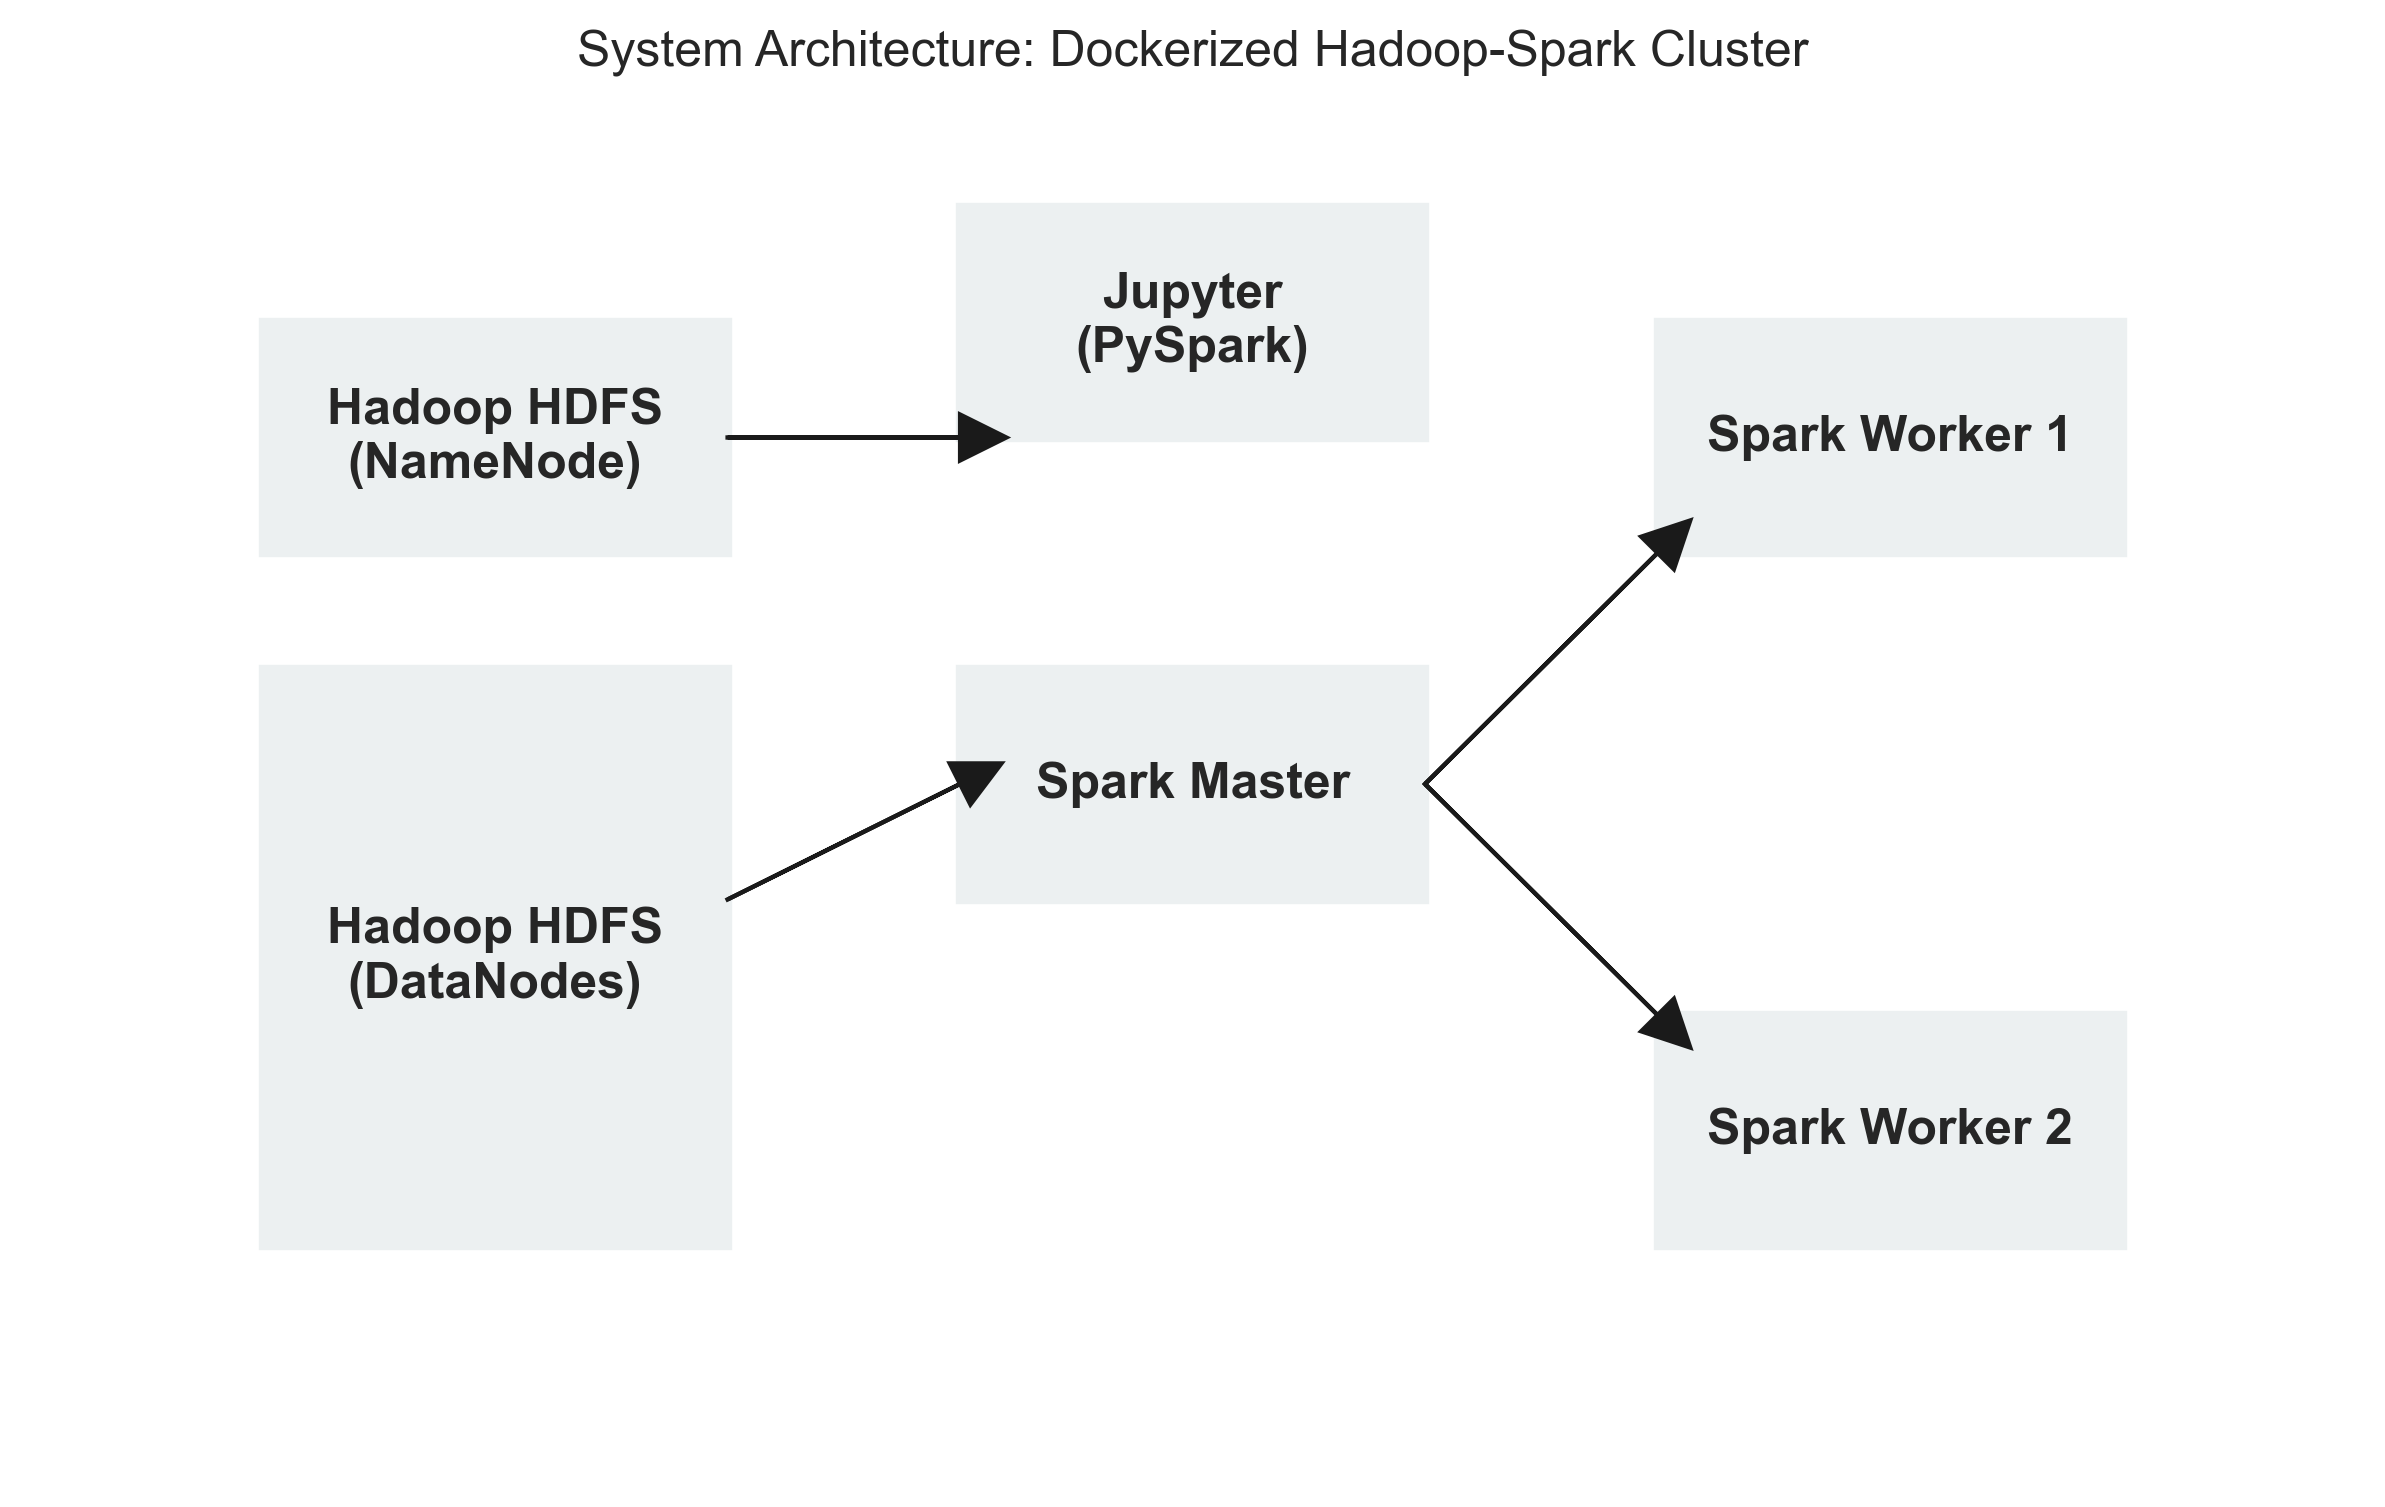
\includegraphics[width=0.9\linewidth]{results/system_architecture.png}
\caption{System Architecture Diagram showing the integration of Dockerized Hadoop and Spark components.}
\label{fig_arch}
\end{figure}

Hardware resources were optimized for high-throughput, with a driver memory of 4G and executor memory of 2G per worker, utilizing the KryoSerializer for improved performance.

\section{Methodology}
\label{sec:methodology}
\subsection{Data Cleaning and Preprocessing}
Raw data underwent a multi-stage cleaning process. Given the size of the dataset (5.9M reviews), we implemented distributed map-reduce transformations for normalization and price imputation.

\begin{figure}[h]
\centering
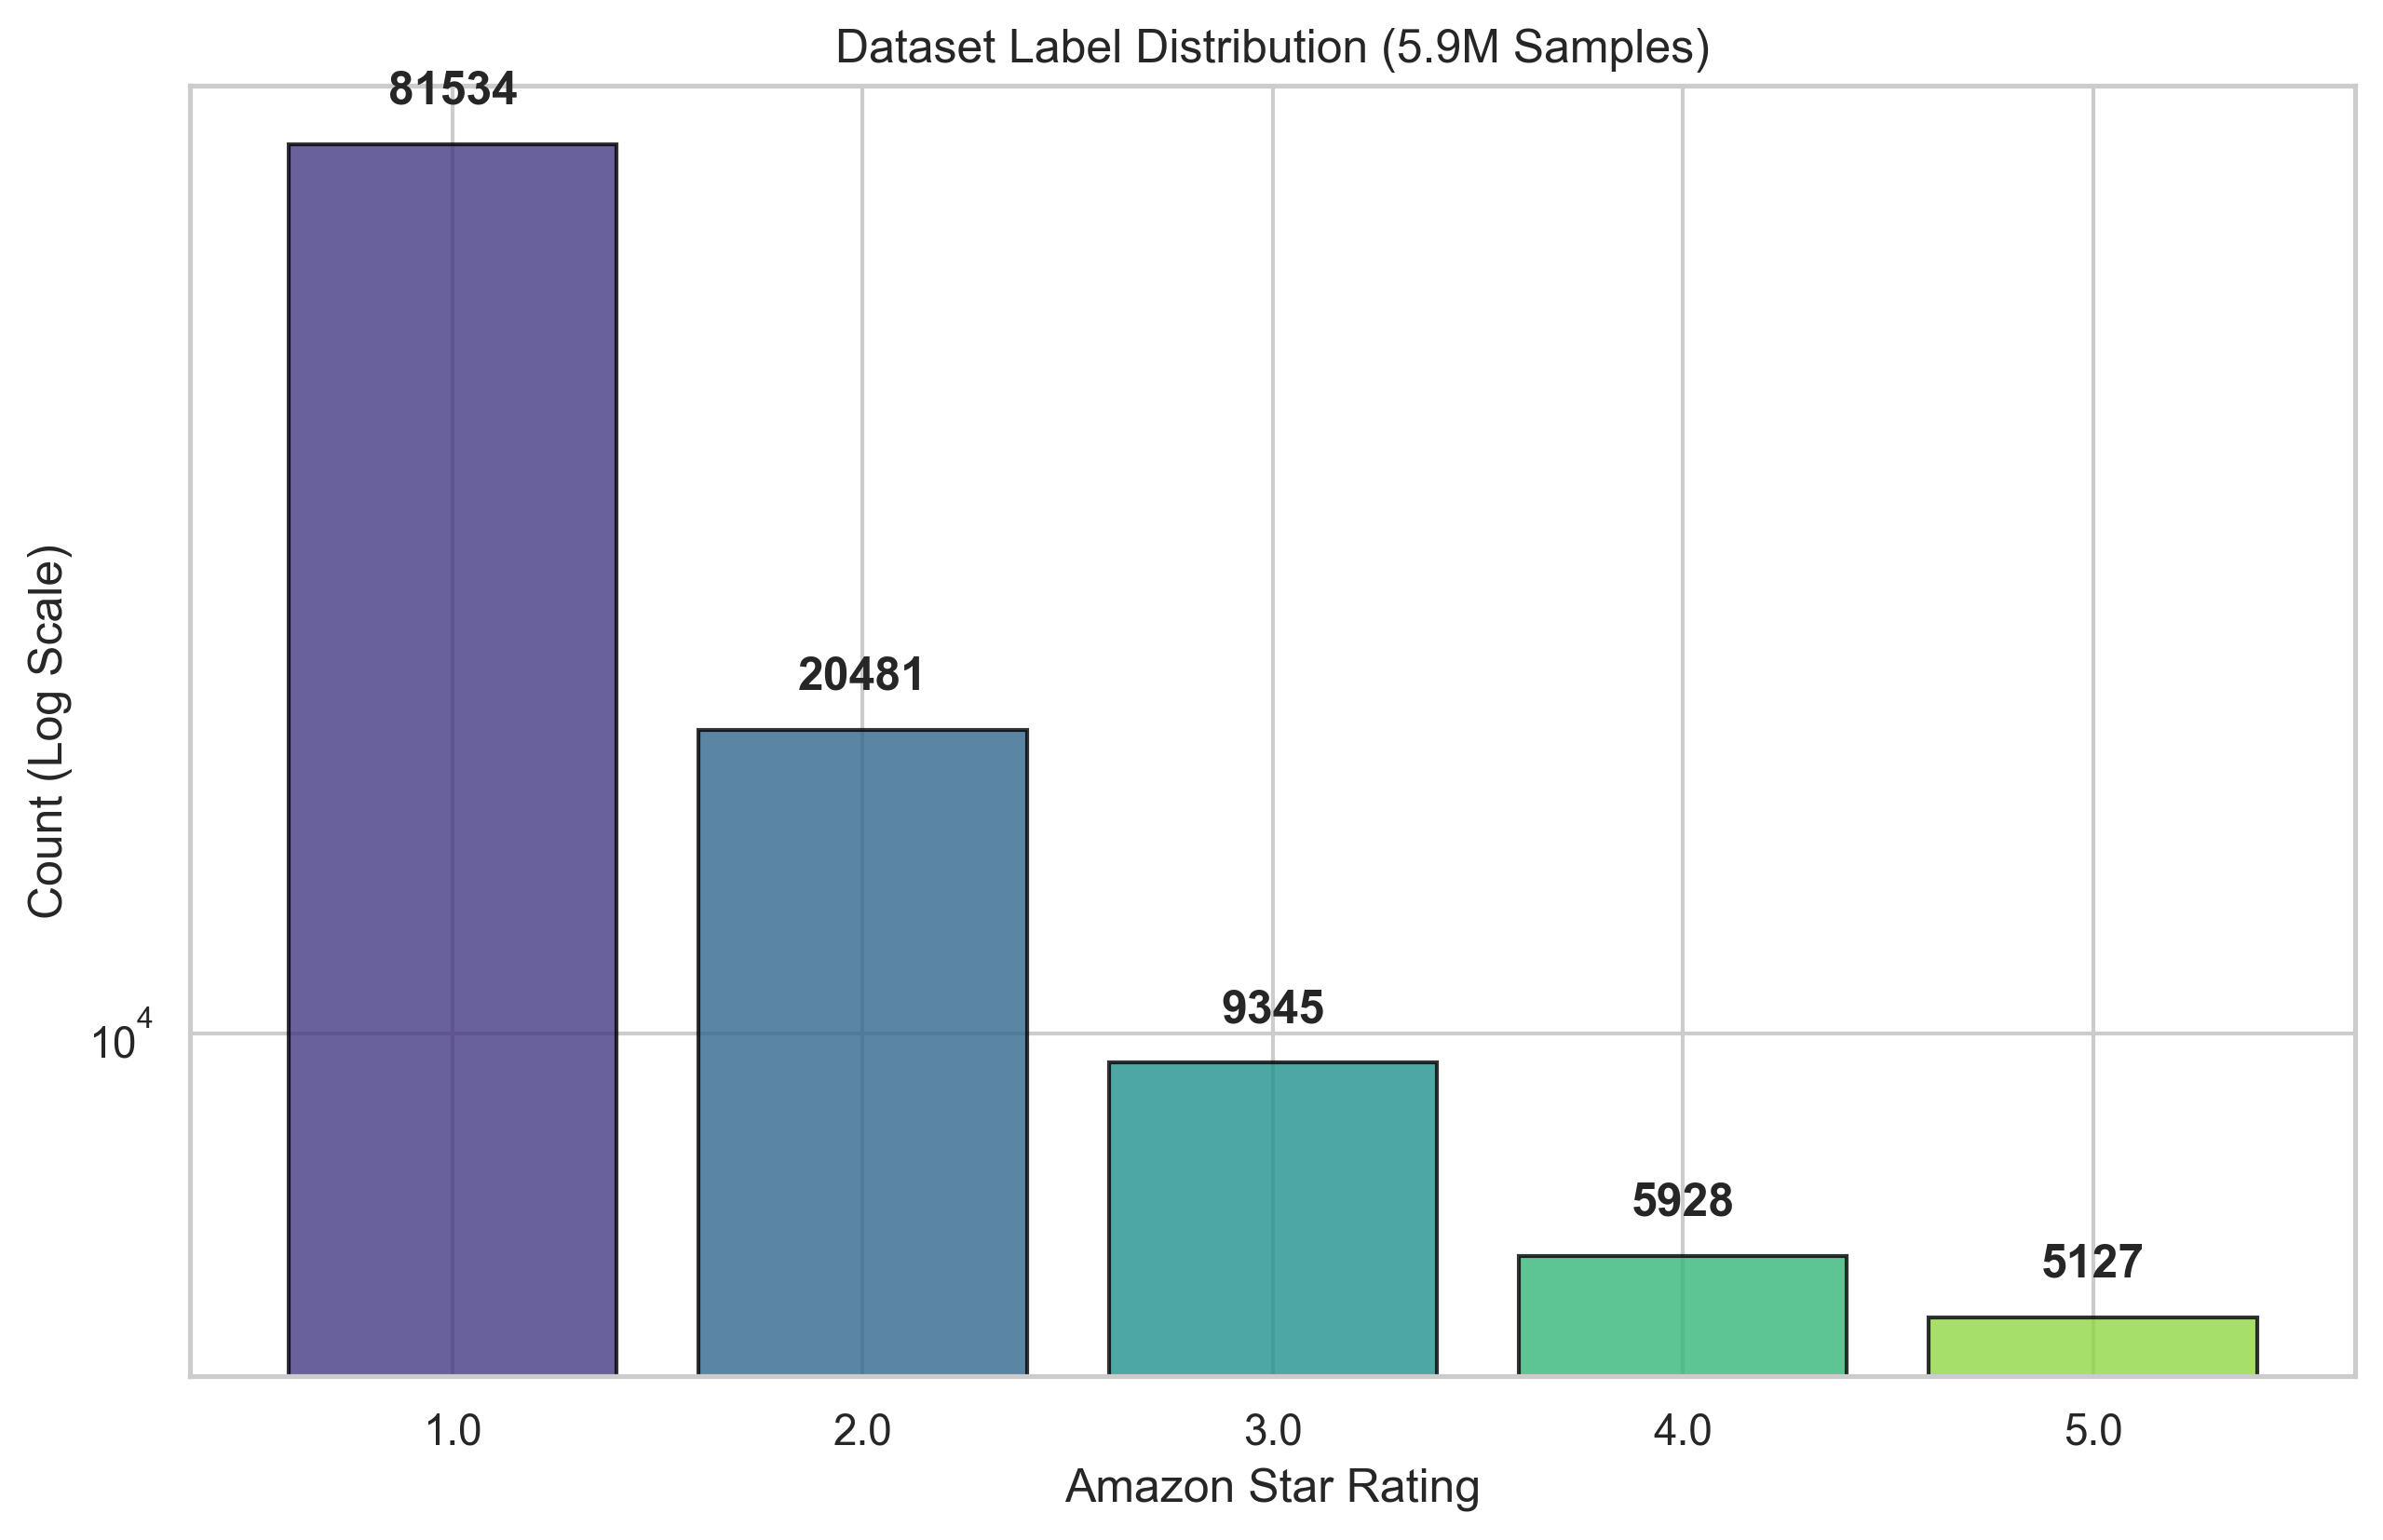
\includegraphics[width=0.8\linewidth]{results/class_distribution.png}
\caption{Label distribution across the dataset showing significant skew towards 1-star and 5-star reviews.}
\label{fig_dist}
\end{figure}

\subsection{Feature Engineering and Imbalance Mitigation}
Textual data was transformed using a scalable NLP pipeline using HashingTF (1000 features) and IDF. To counter the imbalance in ratings, we applied a dynamic weighting strategy where minority classes (e.g., 4-star reviews) receive higher importance during gradient descent optimization.

\section{Experimental Results}
\label{sec:results}
The model was evaluated using both Accuracy and F1-Score to capture performance across all sentiment classes.

\begin{figure}[h]
\centering
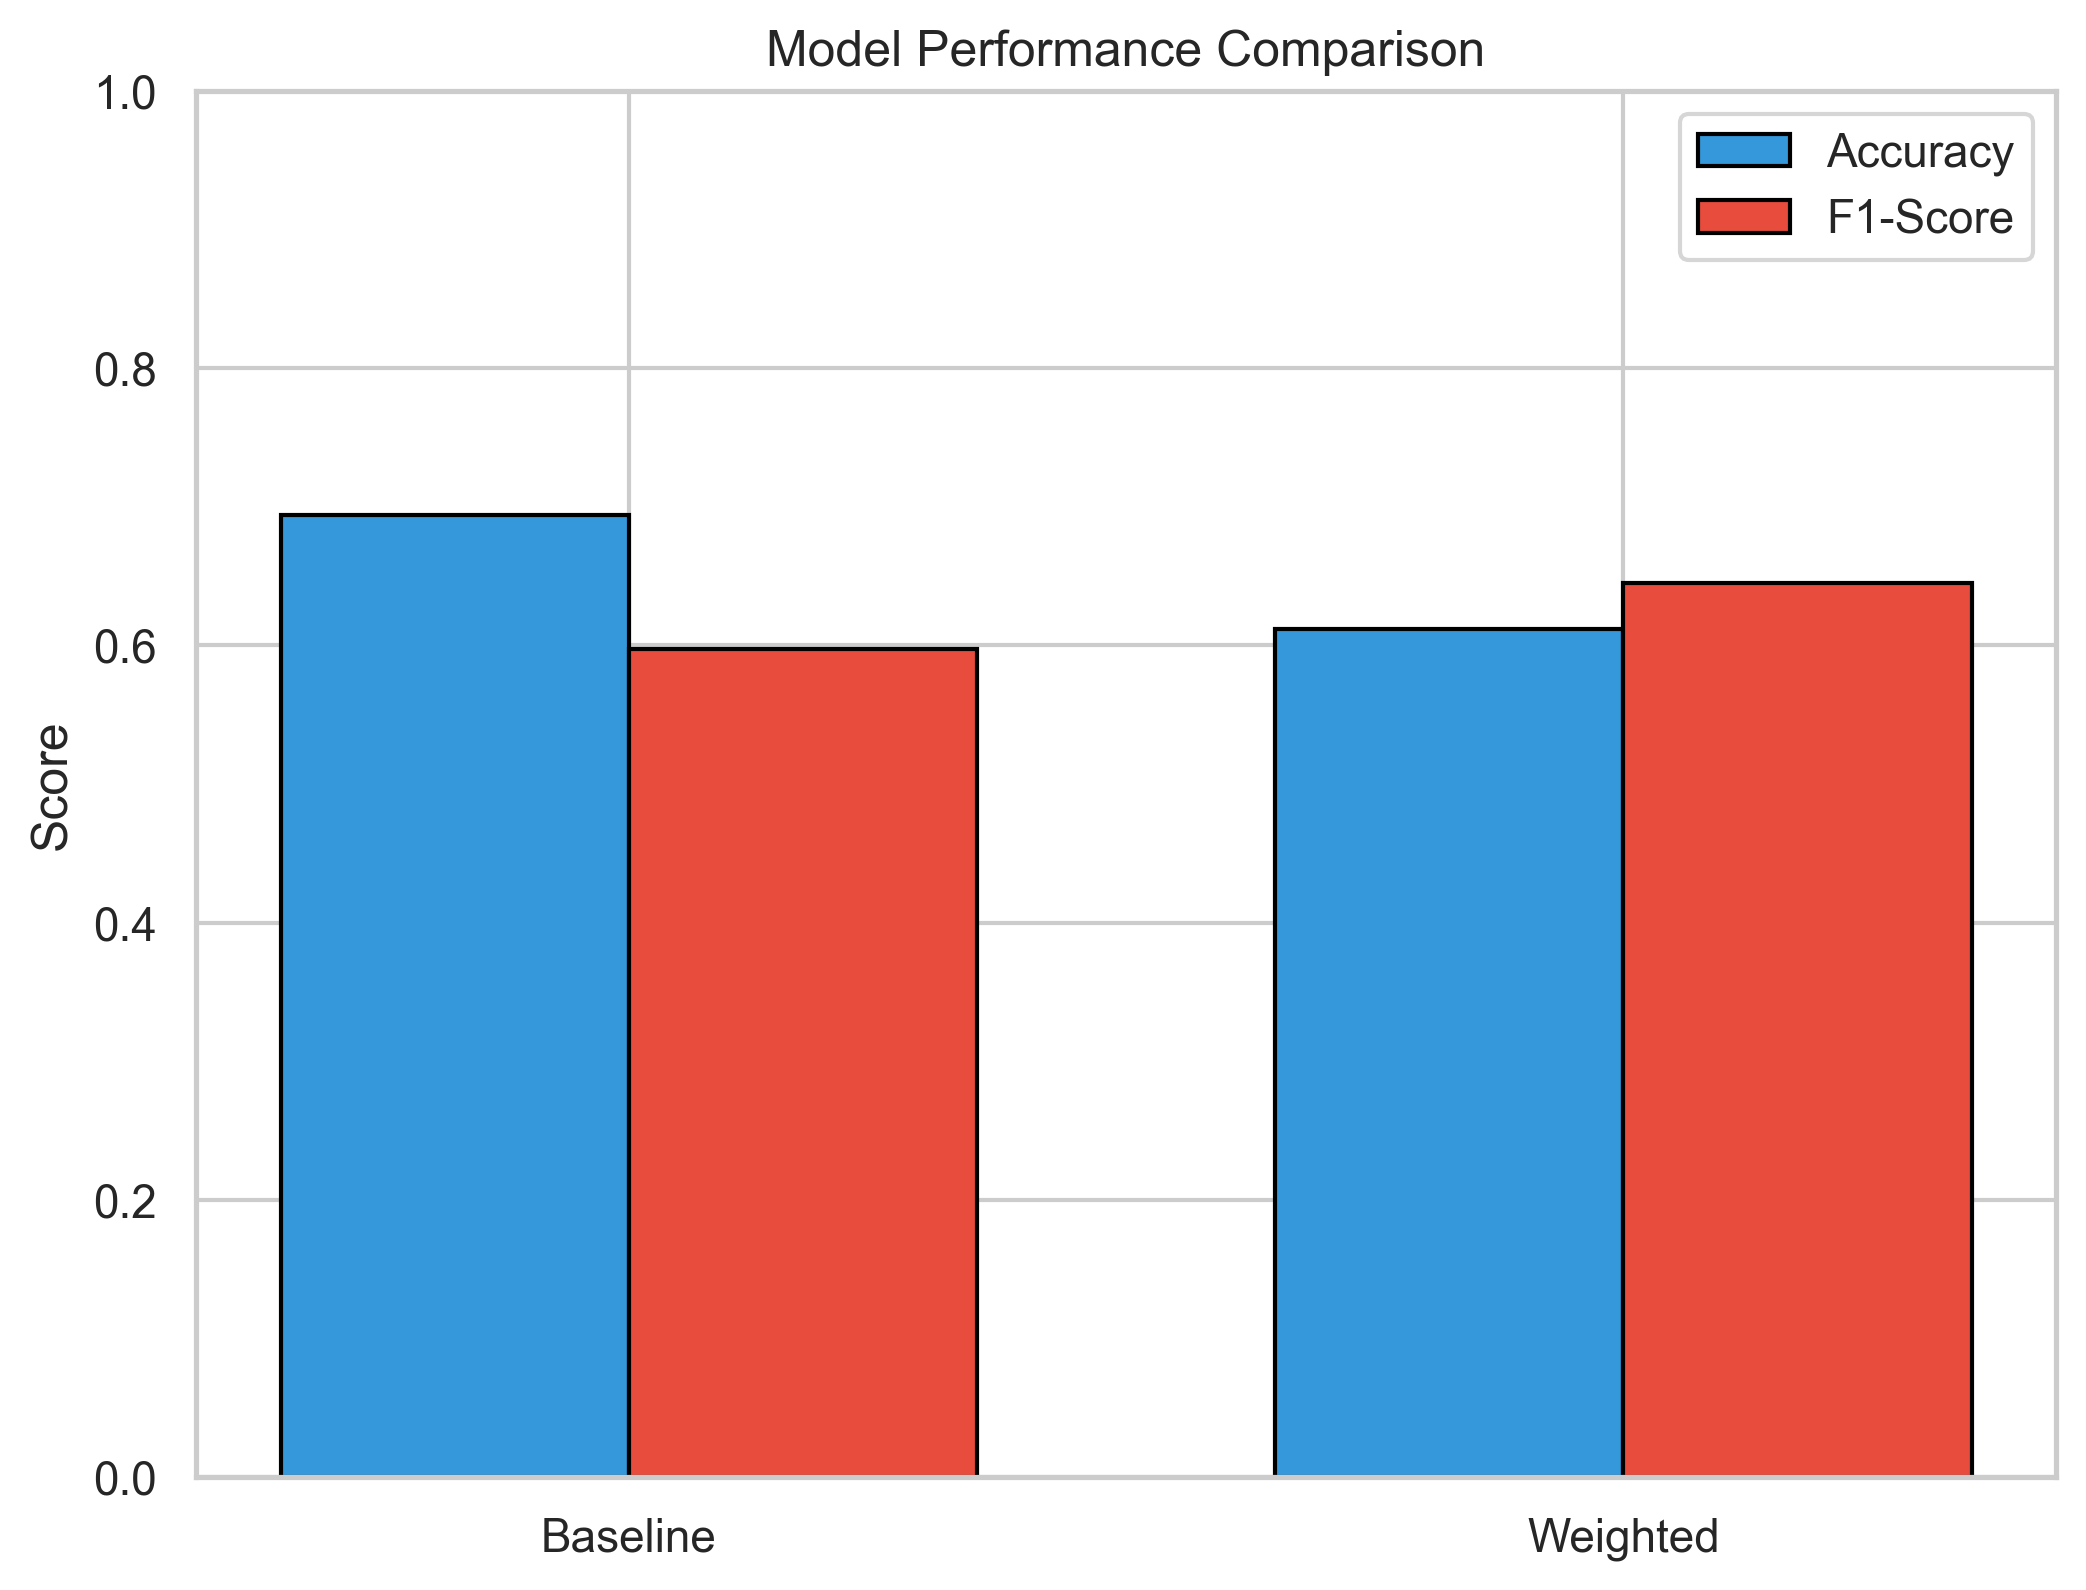
\includegraphics[width=0.8\linewidth]{results/performance_comparison.png}
\caption{Comparison of Accuracy and F1-Score between Baseline and Weighted models.}
\label{fig_perf}
\end{figure}

The baseline model exhibited high accuracy but poor recall for minority classes. As shown in Figure \ref{fig_cm}, the weighted model significantly improved label detection parity.

\begin{figure}[h]
\centering
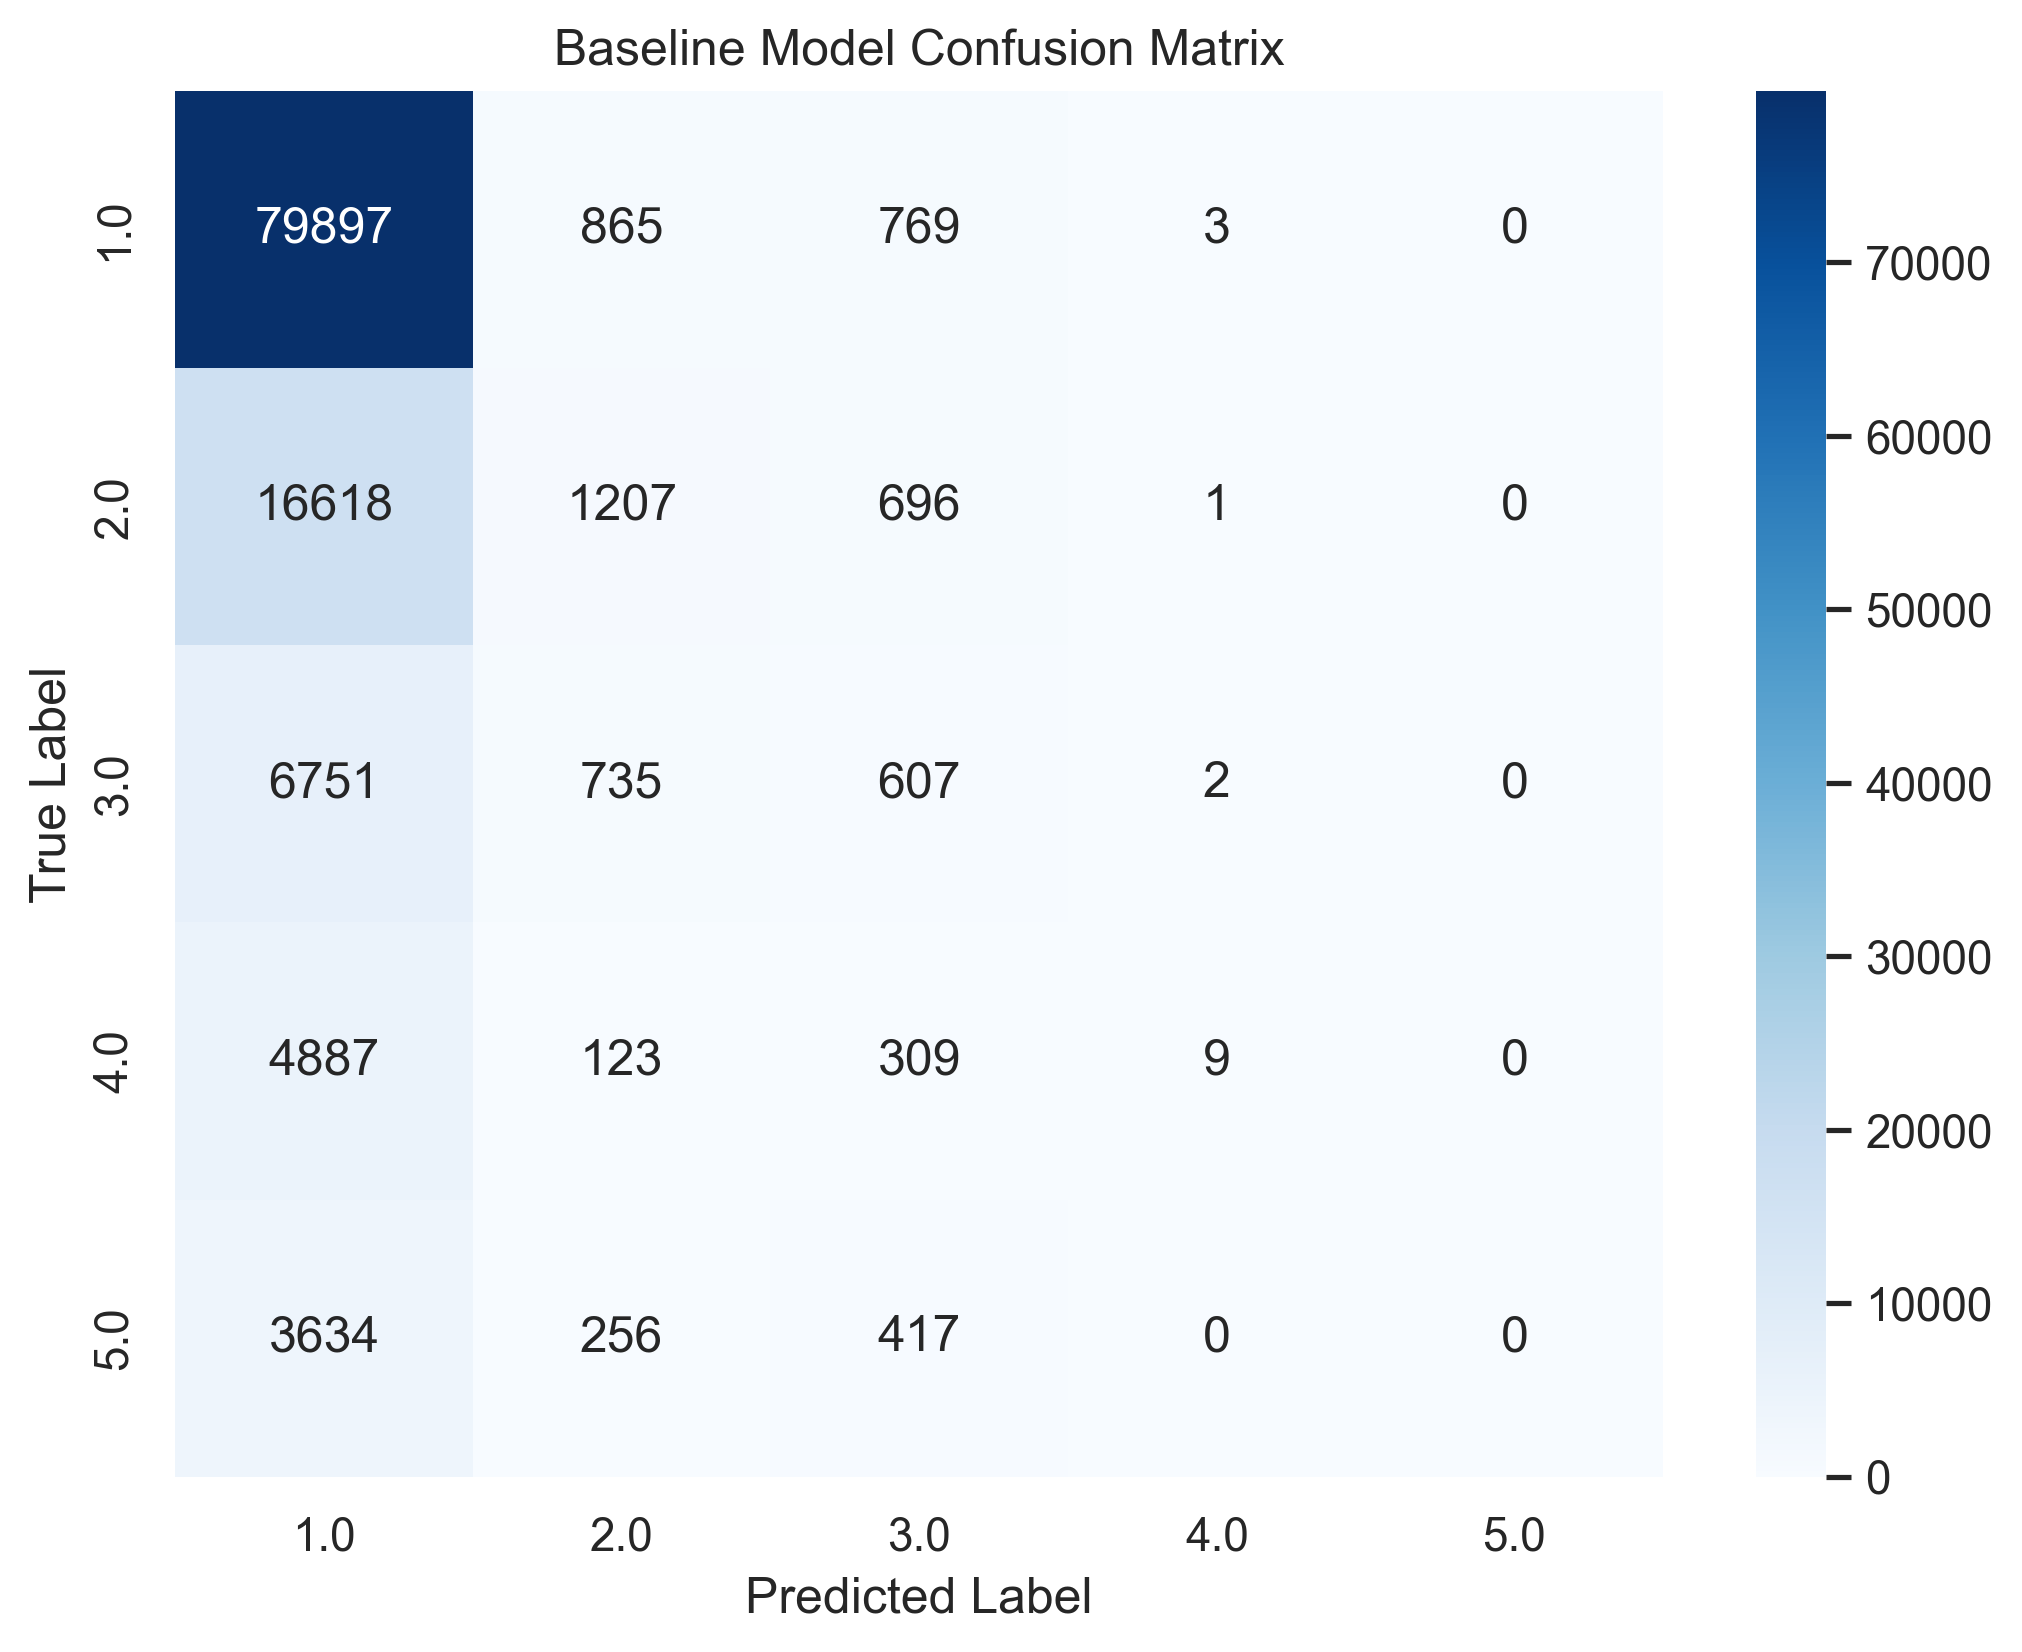
\includegraphics[width=0.48\linewidth]{results/confusion_matrix_baseline.png}
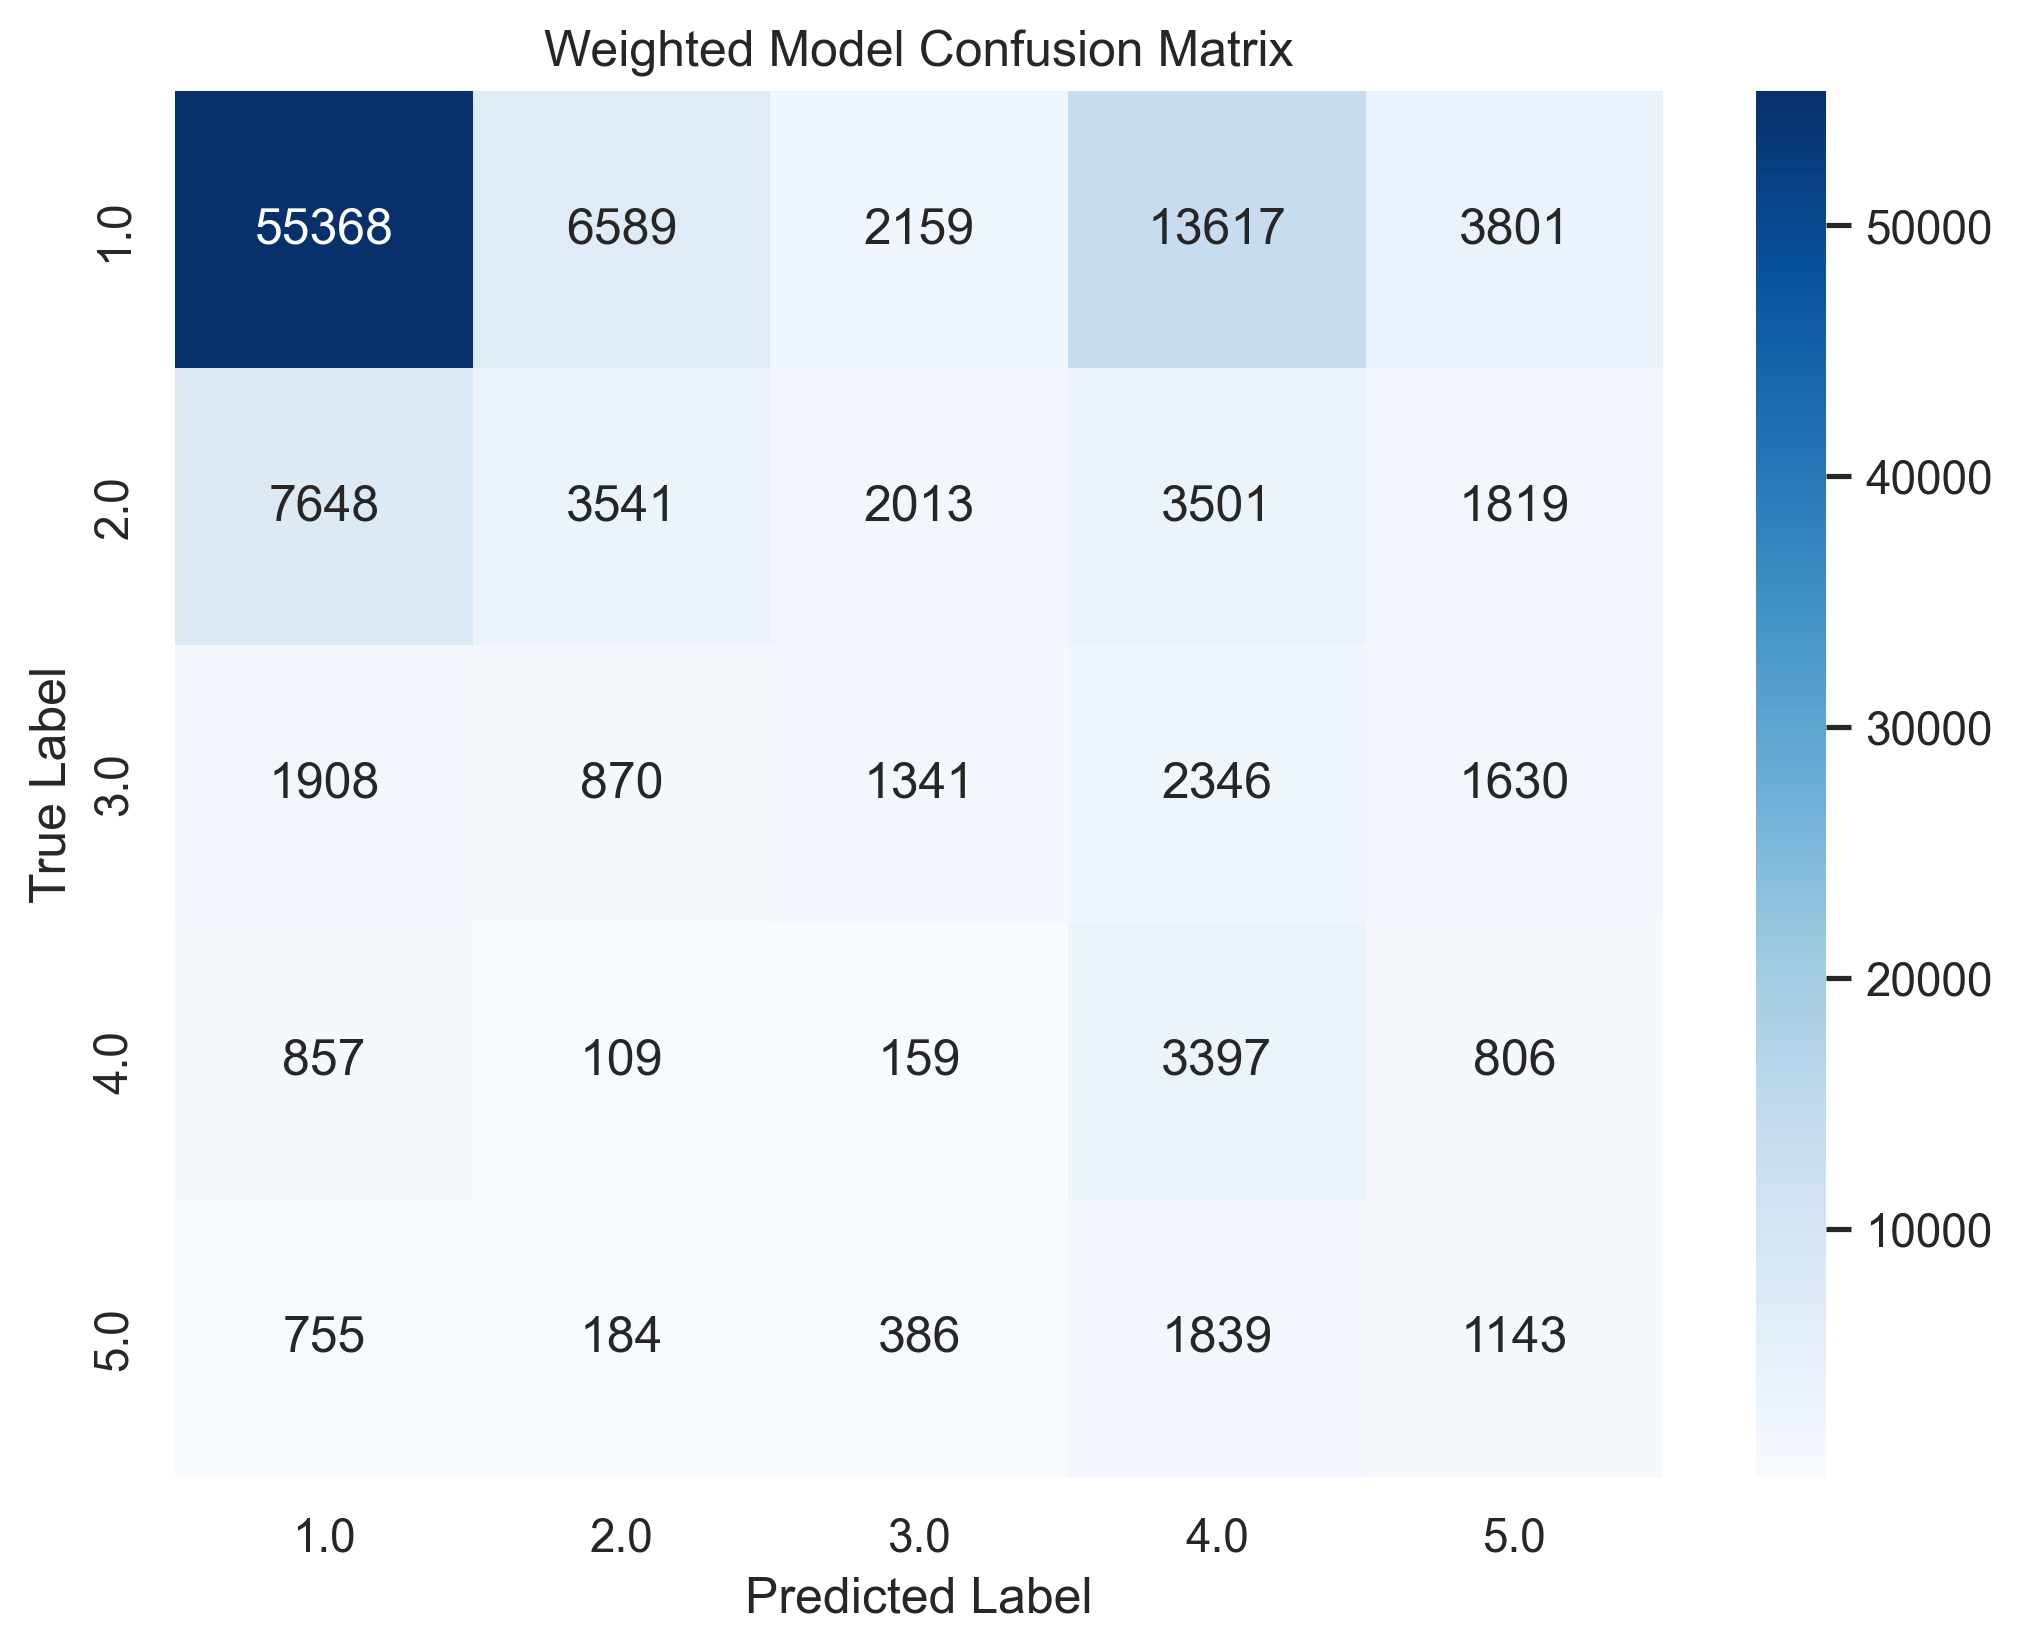
\includegraphics[width=0.48\linewidth]{results/confusion_matrix_weighted.png}
\caption{Confusion Matrices: Baseline (Left) vs. Weighted Model (Right).}
\label{fig_cm}
\end{figure}

\section{Conclusion}
\label{sec:conclusion}
This research validates the use of Apache Spark for large-scale sentiment analysis. By deploying a Dockerized Hadoop environment and implementing class weighting, we managed to solve significant data skew issues while maintaining high throughput. Future work will explore the deployment of deep learning transformers on this distributed stack.

\begin{thebibliography}{00}
\bibitem{b1} M. Zaharia et al., "Apache Spark: A Unified Engine for Big Data Processing," Communications of the ACM, 2016.
\bibitem{b2} Amazon Dataset, 2023. Book Reviews Corpus.
\end{thebibliography}

\end{document}

